\documentclass[10pt,a4paper]{article}
\bibliographystyle{ACM-Reference-Format}
\usepackage[colorlinks=true, urlcolor=blue, linkcolor=red]{hyperref}
\hypersetup{colorlinks=true}
\usepackage{graphicx}
\graphicspath{ {./images/} }

\title{}
\author{Antonio Facchiano\\Salvatore Ruocco\\Simone Vittoria}
\date{10 Gennaio 2024}

\renewcommand\contentsname{Indice}

\begin{document}
	\begin{figure}
		\centering
		
\includegraphics[scale=0.5]{icon}
	\end{figure}
	
	\maketitle
	\newpage
	{
		\hypersetup{linkcolor=black}
		\tableofcontents
	}
	\newpage
	\section{Introduzione}
	\subsection{Ruzzle}
	Ruzzle è un videogioco sviluppato da \href{https://www.maginteractive.com}{MAG Interactive}, rilasciato nel Marzo del 2012 sugli store di Android e iOS.\\
	Il meccanismo di gioco è ispirato ai giochi da tavolo \textit{Il Paroliere} e \textit{Scarabeo}.\\
	Ciascuna partita è divisa in tre round, e il punteggio finale è dato dalla somma dei punteggi ottenuti nei singoli round. In ciascun round il giocatore ha due minuti a disposizione per formare il maggior numero di parole di senso compiuto con le sedici lettere a disposizione nella \textbf{griglia 4x4} sullo schermo. Le parole devono essere di almeno 2 lettere e devono essere formate unendo lettere adiacenti fra loro in orizzontale, verticale o diagonale. Non è possibile inserire la stessa casella-lettera più volte all'interno della stessa parola.\\
	Come nello \textit{Scarabeo}, a ciascuna lettera è assegnato un punteggio in base alla difficoltà di inserirla all'interno di parole di senso compiuto; ad esempio vocali comuni come A, E, I, O valgono 1 punto, mentre le consonanti più rare come la Z o la H valgono 8 punti.\\
	Il punteggio totale assegnato a ciascuna parola trovata è dato dalla somma dei punteggi assegnati alle singole lettere più un "bonus lunghezza" per le parole più lunghe di cinque lettere. È possibile aumentare il proprio punteggio utilizzando le lettere contrassegnate da simboli-bonus: DL duplica il valore relativo alla lettera, TL triplica il suo valore; DW duplica e TW triplica il valore totale della parola. Il numero delle lettere bonus varia a seconda del round: nel primo round sono presenti solamente una DL e una TL, nel secondo round compare anche una DW mentre nel terzo sono presenti anche due DW e una TW. 
	\subsection{Obiettivi}
	Lo scopo di questo progetto è quello di creare un'IA capace di trovare tutte le parole italiane di senso compiuto contenute in una griglia 4x4 di caratteri data in input.
	Quindi restituire in output le parole trovate e le coordinate all'interno della griglia.\\
	Al momento, abbiamo deciso di non dare un peso a ciascuna parola trovata, quindi non assegniamo a loro un punteggio.
	\subsection{Specifica PEAS}
	Un ambiente viene generalmente descritto tramite la specifica PEAS, ovvero \textbf{P}erformance, \textbf{E}nvironment, \textbf{A}ctuators, \textbf{S}ensors.
	\begin{itemize}
		\item \textbf{P}: sono le misure di prestazione adottate per valutare l’operato di un agente, in questo caso vogliamo che l'agente sia completo e veloce.
		\item \textbf{E}: descrizione degli elementi dell'ambiente. Il nostro ambiente è una griglia 4x4 dove ogni casella è un carattere dell'alfabeto italiano.
		\item \textbf{A}: gli attuatori a disposizione dell'agente per intraprendere le azioni. In questo caso i nostri attuatori sono le otto direzioni: nord, nord-est, est, sud-est, sud, sud-ovest, ovest, nord-ovest.
		\item \textbf{S}: i sensori attraverso i quali riceve gli input percettivi.
	\end{itemize}
	\subsection{Caratteristiche dell'ambiente}
	\begin{itemize}
		\item \textbf{Parzialmente osservabile}: l'agente non conosce a priori le coordinate di un carattere, ma data una coordinata, può conoscere il carattere contenuto in quel punto della griglia.
		\item \textbf{Deterministico}: lo stato successivo dell’ambiente è completamente determinato dallo stato corrente e dall’azione eseguita dall’agente.
		\item \textbf{Episodico}: l’esperienza dell’agente è divisa in “episodi” atomici, dove ciascun episodio consiste nell’eseguire una singola azione.
		\item \textbf{Statico}: l'ambiente non muta durante l'esecuzione dell'agente.
		\item \textbf{Discreto}: l’ambiente fornisce un numero limitato di percezioni e azioni distinte, chiaramente definite.
		\item \textbf{Singolo agente}: l'ambiente consente la presenza di  un singolo agente con lo scopo di trovare tutte le parole di senso compiuto possibili.
	\end{itemize}
	\subsection{Formulazione del problema}
	\begin{itemize}
		\item \textbf{Stato iniziale}: griglia 4x4 dove ogni casella contiene una lettere dell'alfabeto italiano.
		\item \textbf{Azioni}: otto direzioni: nord, nord-est, est, sud-est, sud, sud-ovest, ovest, nord-ovest. Queste non sono sempre tutte possibili nel caso in cui ci troviamo ai limiti della griglia, oppure la casella corrispondente è stata già visitata.
		\item \textbf{Modello di transizioni}: ad ogni azione si andrà a controllare se il carattere contenuta nella casella appena visitata è utile per costruire una parola di senso compiuto.
		\item \textbf{Test obiettivo}: trovare tutte le parole di senso compiuto possibili.
		\item\textbf{Costo di cammino}: ogni azione ha lo stesso costo.
	\end{itemize}
	\subsection{Risorse}
	\begin{itemize}
		\item \href{https://github.com/RazzoloDevs/Razzolo}{\textbf{Repository GitHub}}
		\item \textbf{Dizionario italiano} formato da 661563 vocaboli disponibile nella cartella \textit{resources} della repository
	\end{itemize}
	Nel prossimo paragrafo verrano descritti gli algoritmi utilizzati, per ognuno di essi verranno analizzate le prestazioni con i seguenti 4 indicatori:
	\begin{itemize}
		\item \textbf{Completezza}: se la soluzione esiste, l'algoritmo consente di trovarla.
		\item \textbf{Ottimalità}; l'algoritmo garantisce di trovare la soluzione ottima.
		\item \textbf{Complessità temporale}: il tempo impiegato per trovare una soluzione.
		\item \textbf{Complessità spaziale}: la memoria necessaria per trovare una soluzione.
	\end{itemize}
	\newpage
	\section{Ricerca non informata}
	Per raggiungere il nostro scopo, abbiamo deciso di utilizzare degli algoritmi di ricerca non informata.\\
	Questi ultimi fanno riferimento alle strategie di ricerca che \textbf{non dispongono di informazioni aggiuntive sugli stati} oltre a quella fornita nella definizione del problema: tutto ciò che possono fare è generare successori e distinguere gli stati obiettivo dagli altri.\\
	La principale differenza tra le varie strategie di ricerca non informata consiste nell’ordine in cui vengono espansi i nodi.\\
	Data la loro natura, questi algoritmi \textbf{non sanno stimare quanto un nodo non obiettivo sia promettente} per la risoluzione del problema.\\
	Gli algoritmi scelti sono: \textit{ricerca in ampiezza, ricerca in profondità e ricerca ad approfondimento iterativo}.
	\subsection{Ricerca in ampiezza}
	La ricerca in ampiezza è una strategia sistematica di ricerca, ovvero è in grado di \textbf{trovare	sempre una soluzione, se esiste}, nel quale si estende prima il nodo radice e poi i loro successori	e cosi via. In particolare nel nostro caso i nodi vengono espansi attraverso un determinato ordine che sarebbe nord, nord-est, est, sud-est, sud, sud-ovest, ovest, nord-ovest.
	Da un punto di vista pratico, questa strategia può essere implementata utilizzando una semplice \textbf{coda FIFO}. Di conseguenza, i nuovi nodi vanno in fondo alla coda e i nodi vecchi vengono espansi per primi. La ricerca in ampiezza espanderà tutti i nodi che precedono il nodo obiettivo fino a raggiungerlo.\\
	All'algoritmo vengono dati in \textbf{input}: una matrice di caratteri 4x4 e un Set di vocaboli. L'algoritmo restituisce in \textbf{output} una Mappa in cui la chiave è una stringa che rappresenta una parola trovata, ad ogni chiave corrisponde una lista di coordinate.
	Nel nostro caso partirà una ricerca in ampiezza per ogni casella della griglia, quindi in pratica verranno eseguite 16 visite in ampiezza.
	Ad ogni passo, andiamo a verificare se il nodo attauale è un nodo obiettivo, successivamente avviamo un ciclo per esplorare tutti i nodi vicini.\\
	Come conseguenza del fatto che espande tutti i nodi precedenti al nodo obiettivo conosciamo che la sua complessità temporale è O($b^d$) che nel nostro problema si traduce con un fattore di ramificazione b di 8 (le possibili azioni che ad ogni stato può effettuare) e d, che indica la profondità del nodo obiettivo più vicino allo stato iniziale. Mentre dal punto di vista della memoria occupata, ci saranno O($b^d$) nodi nella frontiera.\\
	Completezza ??\\
	Ottimalità ??\\
	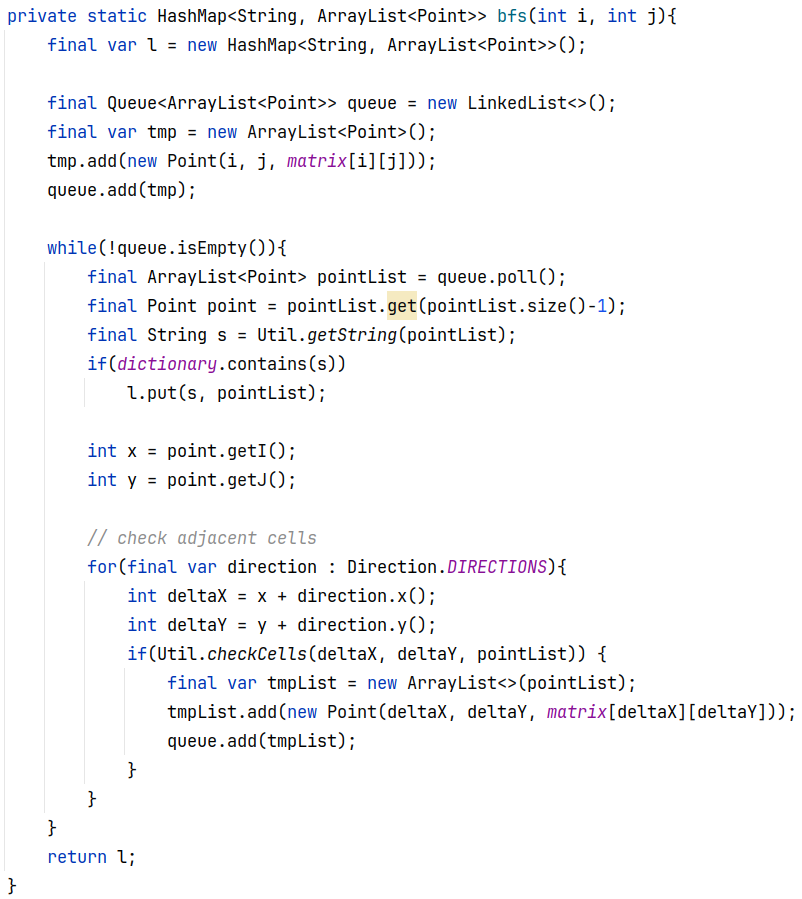
\includegraphics[scale=0.8]{bfs}
	\newpage
	\subsection{Ricerca in profondità}
	La ricerca in profondità fa la stessa cosa della ricerca in ampiezza, ma in modo diverso. Infatti, non espande i nodi come un pendolo ma procede analizzando \textbf{un ramo alla volta della matrice}. Dunque raggiunge immediatamente il livello più profondo della matrice, dove i nodi non hanno successori. L’espansione di tali nodi li rimuove dalla frontiera, per cui la ricerca “torna indietro” (backtracking) per riconsiderare il nodo più profondo che ha successori non ancora espansi. L'implementazione è molto simile a quello della ricerca in ampiezza, solo che la frontiera fa uso di una coda LIFO (Stack), poiché verrà sempre espanso l’ultimo nodo generato. Di questo tipo di ricerca ne esiste anche una versione ricorsiva, in cui lo Stack è implicitamente fornito dalle chiamate ricorsive.\\
	Questo algoritmo presenta dei \textbf{problemi} nel momento in cui l’albero di ricerca ha uno spazio degli stati con profondità infinita o con cicli, infatti l’algoritmo non terminerà. Quindi, possiamo sostenere che l’algoritmo di ricerca in profondità non è completo.
	Ma in questo caso, l'albero di ricerca è rappresentato da una matrice di cardinalità finita, che evita stati ripetuti e cammini ridondanti, quindi la ricerca è completa, se la soluzione esiste, perché alla fine espanderà tutti i nodi.\\
	La complessità temporale resta uguale a quello della ricerca in ampiezza, ovvero  O($b^m$) , dove m è la profondità massima di un nodo. Mentre lo spazio occupato è O(m), perché fa uso di backtracking, quindi non avremo mai uno Stack di taglia superiore a m. Da sottolineare che m può essere più grande di d.\\
	\\
	\textit{Non verrà riportato il codice di questo algoritmo essendo simile a quello mostrato precedentemente.}
\end{document}